\chapter{Image processing}
\section{Image processing basics}
\subsection{Example}
\begin{enumerate}
    \item Increasing \transtip{对比度}{contrast} with "S curve", $ouput(x,y)=f(input()x,y)$
    \begin{figure}[H]
        \centering
        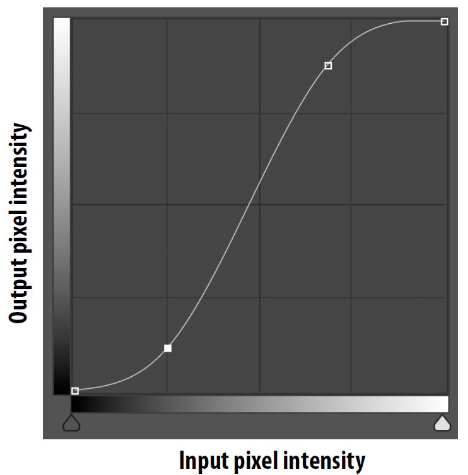
\includegraphics[width=0.38\textwidth]{/Lec3/increasing contrast}
        \caption{Increasing contrast}
    \end{figure}
    \item 整体变亮
    \item \transtip{模糊}{Blur}: 去噪
    \item "smarter" blur
    \item \transtip{锐化}{Sharpen}
    \item \transtip{边缘检测}{Edge detection}
\end{enumerate}
\subsection{Review: convolution}
\begin{align*}
    \overset{\textcolor{red}{\text{output signal}}}{(f*g)(x)}=\int_{-\infty }^{\infty}  \overset{\textcolor{red}{\text{filter}}}{f(y)}\overset{\textcolor{red}{\text{input signal}}}{g(x-y)}\,dy 
\end{align*}

卷积意义: 对输入的每个点,  将其周围的值取出, 并用卷积核相乘, 再积分(离散就直接相加). 

\begin{enumerate}
    \item 卷积核需要翻转(但一般就是对称的所以忽略了翻转). 
    \item 在亮度相差不大的情况下, 图像中与卷积和越相似的地方响应越大. 
\end{enumerate}

\subsection{Discrete 2D convolution}
\begin{align*}
    (f*g)(x,y)=\sum_{i,j=-\infty}^{\infty}\overset{\textcolor{red}{\text{filter}}}{f(i,j)}I(x-i,y-j)
\end{align*}

会让输出变小

\subsection{Padding}
要在图边缘填充像素
\begin{enumerate}
    \item Zero values
    \item Edge values
    \item Symmetric 
\end{enumerate}

eg:
\begin{enumerate}
    \item box blur: 取平均
    \item Gaussian blur: 加权平均
    \begin{align*}
        f(i,j)=\frac{1}{2\pi \sigma^2}e^{-\frac{i^2+j^2}{2\sigma^2}}\\
        \text{The bigger } \sigma \text{ is, the more blurry pic will be.}
    \end{align*}
    \begin{figure}[H]
        \centering
        \includegraphics[width=0.38\textwidth]{/Lec3/Gaussian}
        \caption{Gaussian}
    \end{figure}
    \item Sharpens: 增加对比度
    \begin{align*}
        \begin{bmatrix}
            0&-1&0\\-1&5&-1\\0&-1&0
        \end{bmatrix}
    \end{align*}
    \begin{enumerate}
        \item $I$ is original image: $\begin{bmatrix}
            0&0&0\\0&1&0\\0&0&0
        \end{bmatrix}$. 
        \item High frequencies in image $I=I-blur(I)$, (原本减去低频就是高频)
        \item Sharpened image $=I+(I-bule(I))$. (加强高频)
    \end{enumerate}
    \item Gradient detection filters(梯度边缘检测)
    \begin{enumerate}
        \item Extracts horizontal gradients(检测竖直边缘): $\begin{bmatrix}
            -1&0&1\\-2&0&2\\-1&0&1
        \end{bmatrix}$
        \item Extracts vertical gradients(检测水平边缘): $\begin{bmatrix}
            -1&-2&-1\\0&0&0\\1&2&1
        \end{bmatrix}$
        \begin{figure}[H]
            \begin{subfigure}{0.48\textwidth}
                \centering
                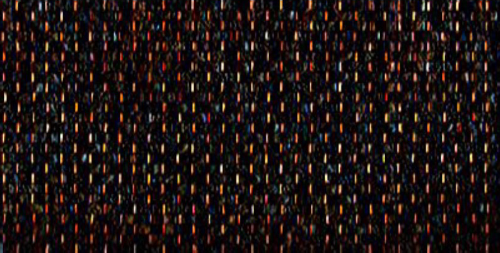
\includegraphics[width=\textwidth]{/Lec3/horizontal}
                \caption{Horizontal gradients}
            \end{subfigure}
            \begin{subfigure}{0.48\textwidth}
                \centering
                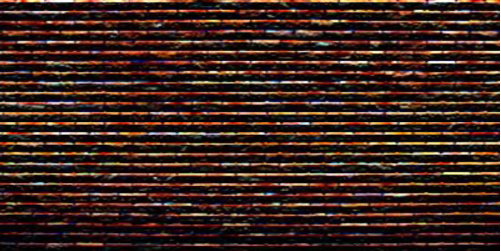
\includegraphics[width=\textwidth]{/Lec3/vertical}
                \caption{Vertical gradients}
            \end{subfigure}
            \caption{Gradient detection filters}
        \end{figure}
    \end{enumerate}
    \item Bilateral filter(双边滤波器): 图像变得更加光滑(去噪), 但保留边缘信息
    \begin{figure}[H]
        \centering
        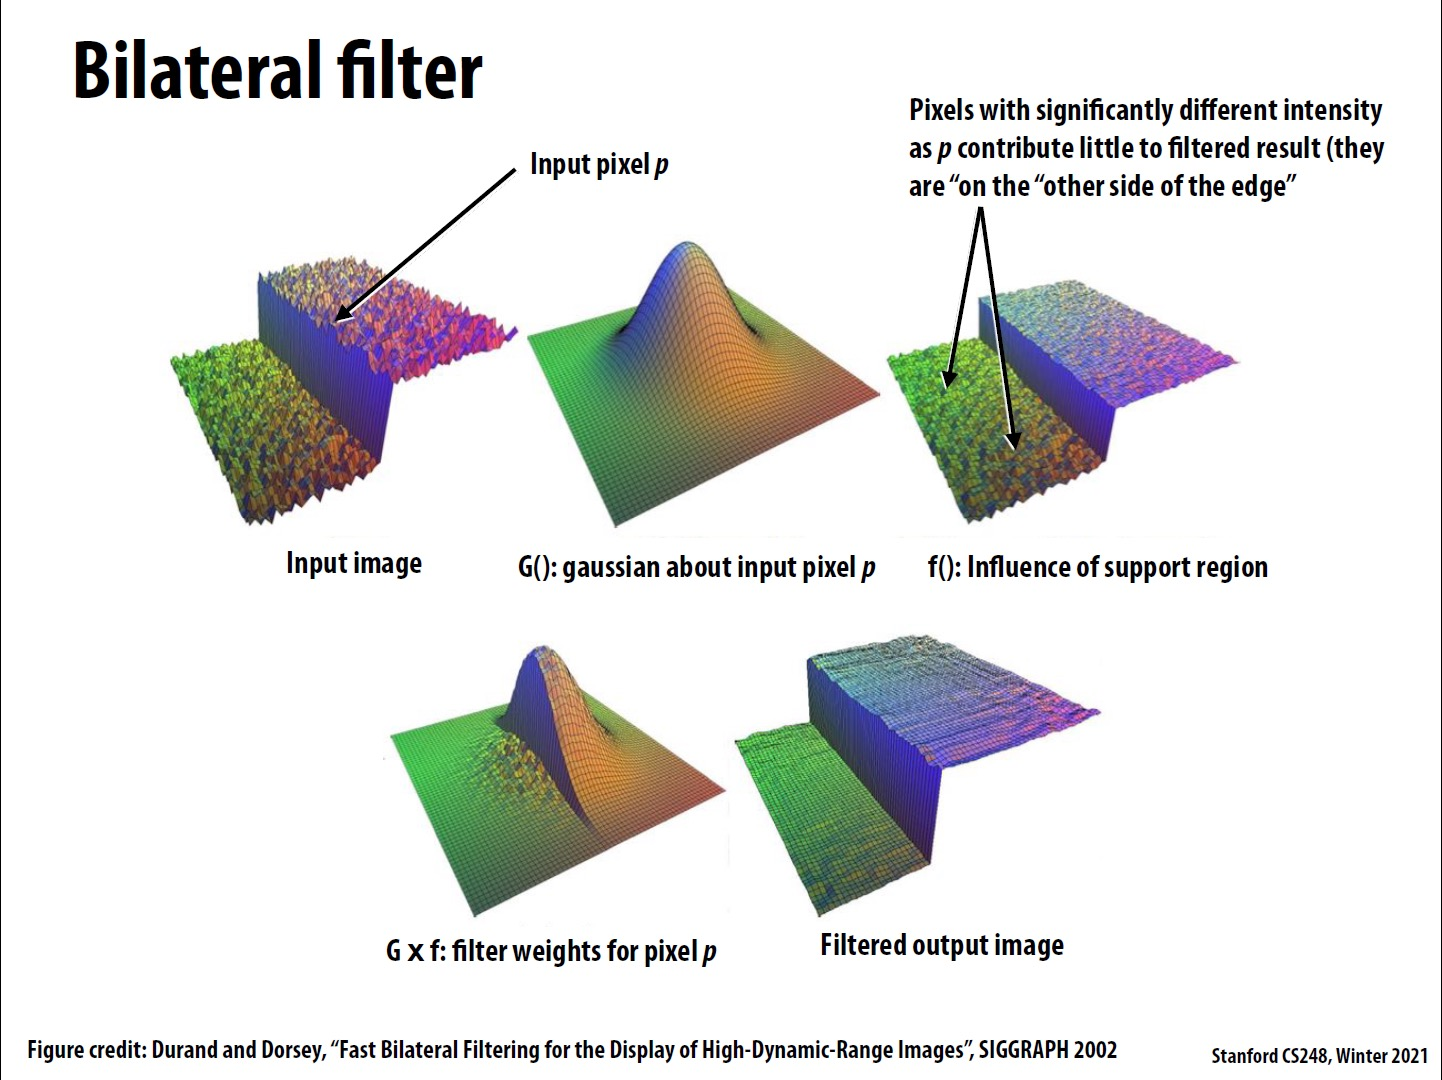
\includegraphics[width=0.38\textwidth]{/Lec3/Bilateral}
        \caption{Bilateral filter}
    \end{figure}
\end{enumerate}

\section{Image sampling(采样)}

\subsection{Image resizing}
\transtip{pixels}{像素}尺寸与\transtip{inches}{物理}尺寸, 物理尺寸有意义需要\transtip{resolution}{分辨率}, 单位: 像素/英寸. 人眼分辨率是300 dip

\subsection{Down-sampling}
Reducing image size. 
\begin{enumerate}
    \item Problem: \transtip{走样}{Aliasing}(artifacts due to sampling)
    \begin{enumerate}
        \item  会出现摩尔纹. 
        \item  Wagon Wheel Illusion(False Motion)
    \end{enumerate}
    \item Reason: Signals are changing too fast but \transtip{采样}{sampled} too slow. 
    \begin{figure}[H]
        \centering
        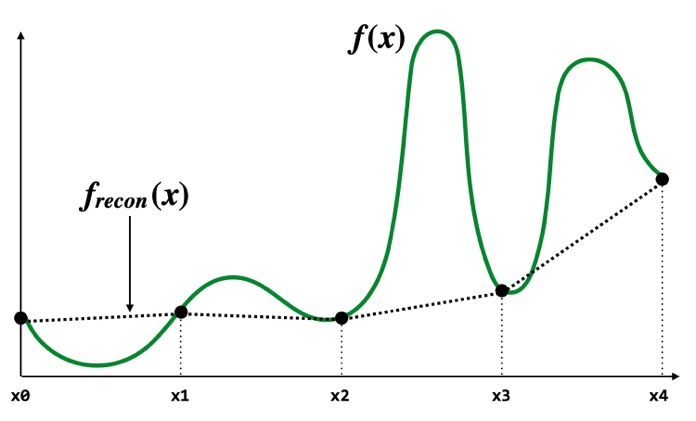
\includegraphics[width=0.38\textwidth]{Lec3/Aliasing}
        \caption{Aliasing}
    \end{figure}
    \item Mathematically describe: $f=\frac{1}{T}$
    \begin{figure}[H]
        \centering
        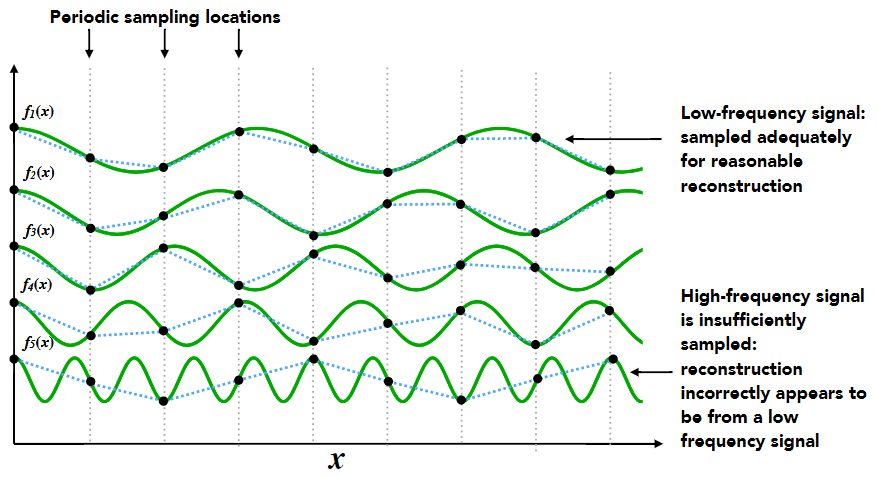
\includegraphics[width=0.6\textwidth]{Lec3/Frequencies}
        \caption{Frequencies \& Sampling}
    \end{figure}

    Higher Frequencies Need Faster Sampling.
\end{enumerate}
\subsection{Fourier Transform}
    Represent a function as a weighted sum of
    sines and cosines. To obtain the frequencies of arbitrary signals. 
     
    \begin{figure}[H]
        \centering
        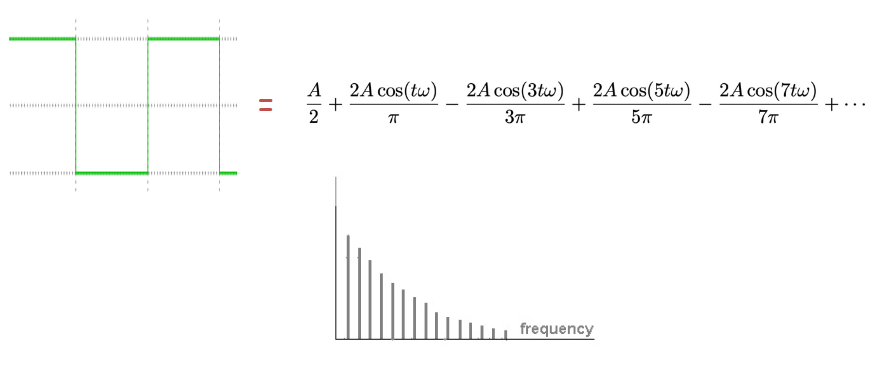
\includegraphics[width=0.6\textwidth]{Lec3/Fourier}
        \caption{Fourier}
    \end{figure}
    \begin{align*}
        x:\text{space}, u: \text{frequency}, e^{i\theta}=\cos\theta+i\sin\theta
    \end{align*}
    \begin{align*}
        F(u)&=\int_{-\infty}^{\infty}f(x)e^{-i2\pi ux}\, dx\\
        f(x)&=\int_{-\infty}^{\infty}F(u)e^{i2\pi ux}\, du
    \end{align*}
    \begin{figure}[H]
        \centering
        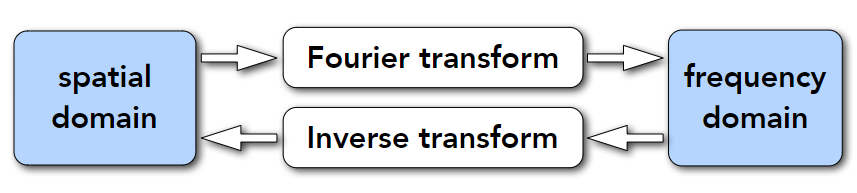
\includegraphics[width=0.38\textwidth]{Lec3/Fourier Transform}
        \caption{Fourier Transform}
    \end{figure}

    对Fourier Transform的频率而言, 中间频率低, 两边频率高.

    频率大小对应在这个频率下$\sin \cos$与原图像拟合的多少? 也可以看作原图像变化的速度. 
    
    频域信号$F(u)$代表原来的信号在$u$频率上的大小.

    二维频谱$F(u,v)$, 代表原来信号沿x,y两个方向分别在$u,v$频率上的大小. (并不与原坐标相对应)

   

    \begin{figure}[H]
        \centering
        \caption{Examples(一维)}
        \begin{subfigure}{0.18\textwidth}
            \centering
            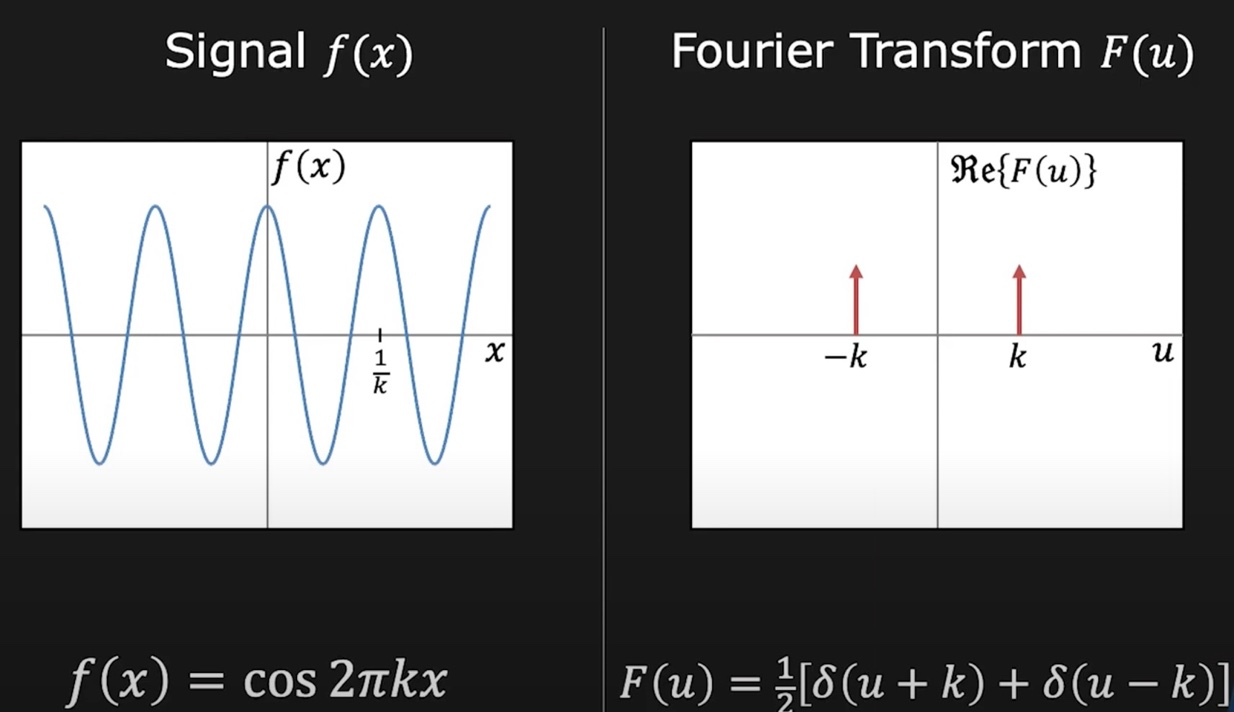
\includegraphics[width=\textwidth]{Lec3/cos}
            \caption{cosinusoids \\(余弦信号)}
        \end{subfigure}
        \begin{subfigure}{0.18\textwidth}
            \centering
            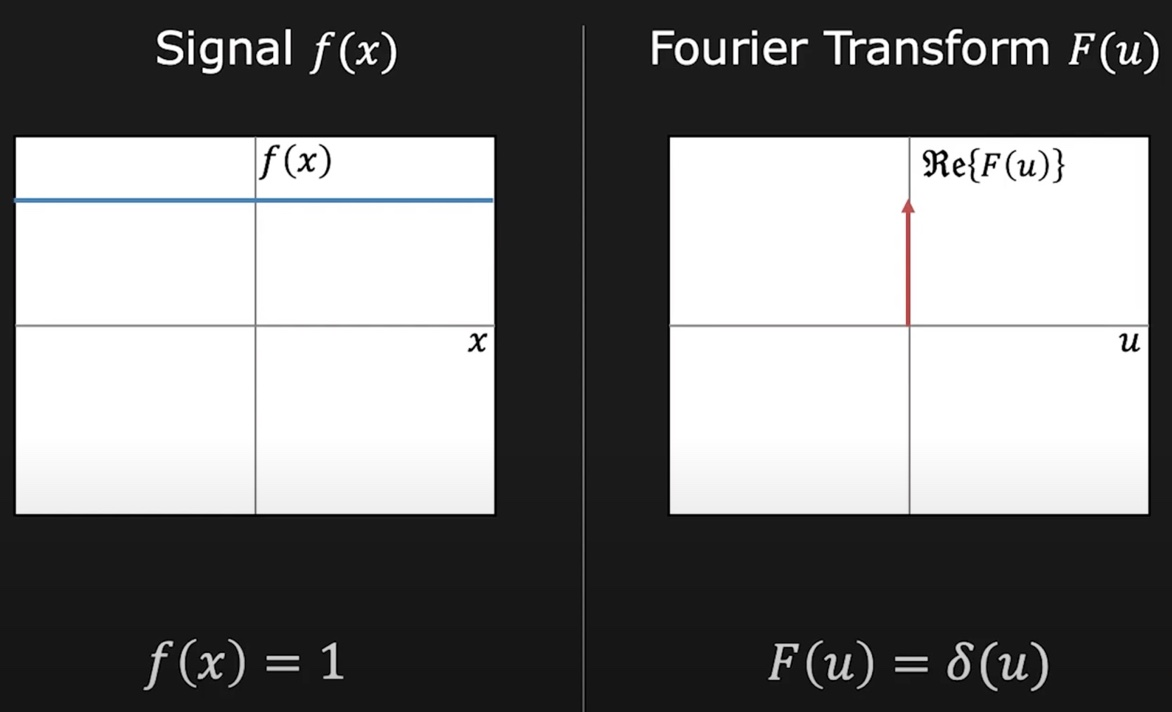
\includegraphics[width=\textwidth]{Lec3/constant}
            \caption{Constant function\\ (常数)}
        \end{subfigure}
        \begin{subfigure}{0.18\textwidth}
            \centering
            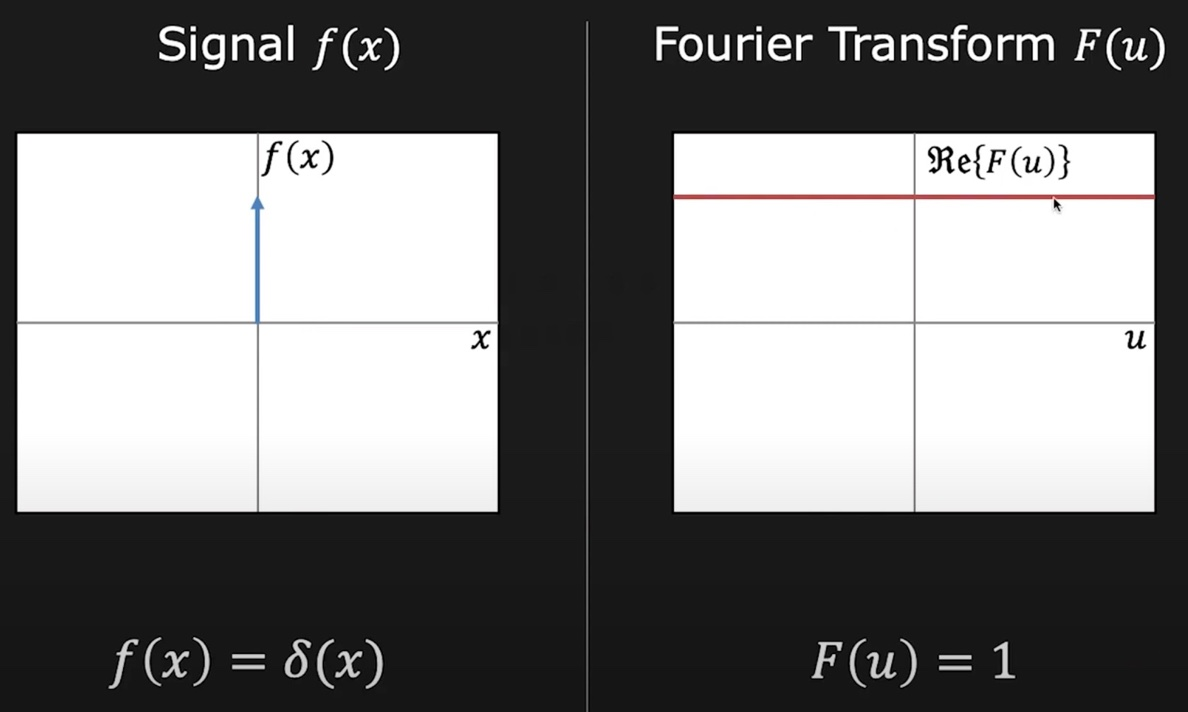
\includegraphics[width=\textwidth]{Lec3/Dirac}
            \caption{Dirac function \\($\delta $, 冲击信号)}
        \end{subfigure}
        \begin{subfigure}{0.18\textwidth}
            \centering
            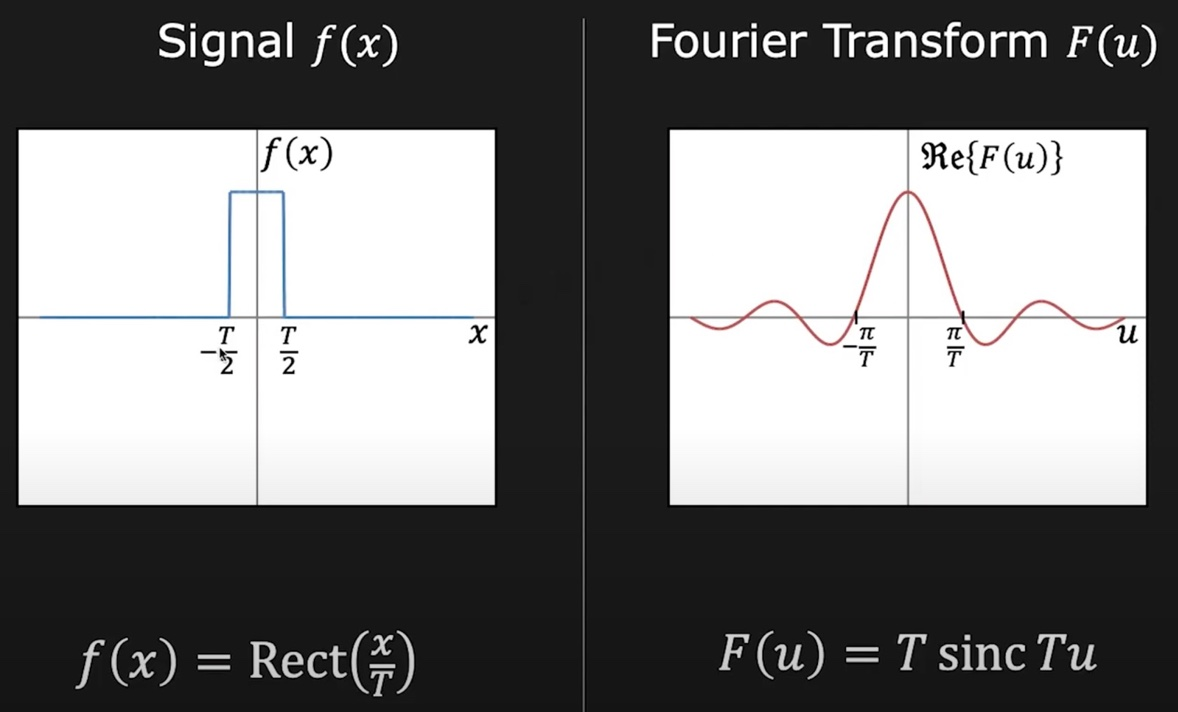
\includegraphics[width=\textwidth]{Lec3/box}
            \caption{Box function \\(窗口)}
        \end{subfigure}
        \begin{subfigure}{0.18\textwidth}
            \centering
            \includegraphics[width=\textwidth]{Lec3/Gaussian.jpg}
            \caption{Gaussian \\(二者都是Gaussian)}
        \end{subfigure}
    \end{figure}
    
    Convolution Theorem(卷积定理)
    \begin{alignat*}{2}
        \overset{\text{空间域}}{\text{Spatial Domain}}&&\overset{\text{频域}}{\text{Frequency Domain}}\\
        \underset{\text{Convolution}}{g(x)=f(x)*h(x)} &\Longleftrightarrow & \underset{\text{Multiplication}}{ G(u)=F(u)H(u)}\\
        \underset{\text{Multiplication}}{g(x)=f(x)h(x)} &\Longleftrightarrow & \underset{\text{Convolution}}{ G(u)=F(u)*H(u)}
    \end{alignat*}
    二维也成立

    \begin{figure}[H]
        \centering
        \caption{Examples(二维)}
        \begin{subfigure}{0.24\textwidth}
            \centering
            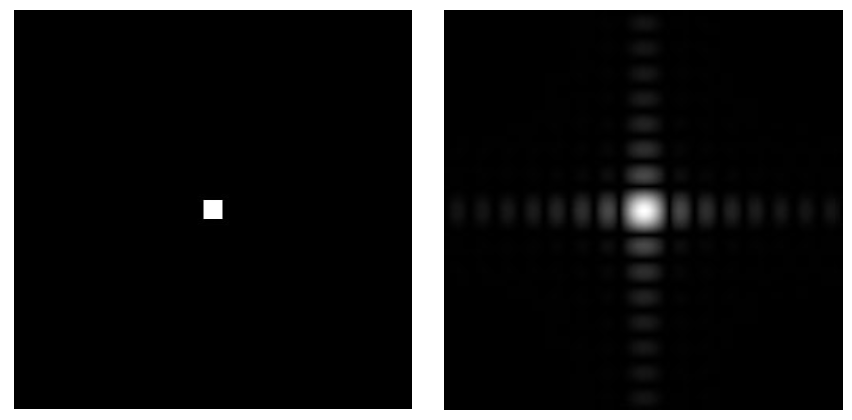
\includegraphics[width=\textwidth]{Lec3/Box filter}
            \caption{Box filter=low-pass filter\\(均值滤波器)}
        \end{subfigure}
        \begin{subfigure}{0.24\textwidth}
            \centering
            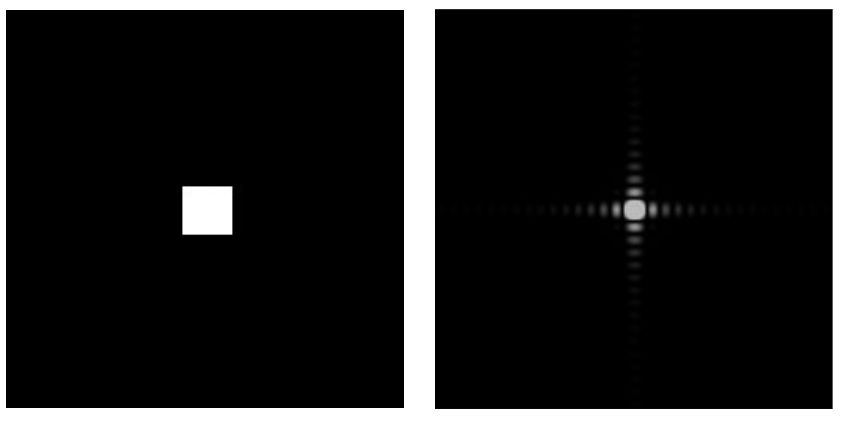
\includegraphics[width=\textwidth]{Lec3/Wider kernel}
            \caption{Box filter\\(Wider kernel=lower frequency)}
        \end{subfigure}
    \end{figure}

    \subsection{Sampling}
    Sampling a signal = multiply the single by \transtip{脉冲信号}{a Dirac comb function}.
    \begin{figure}[H]
        \centering
        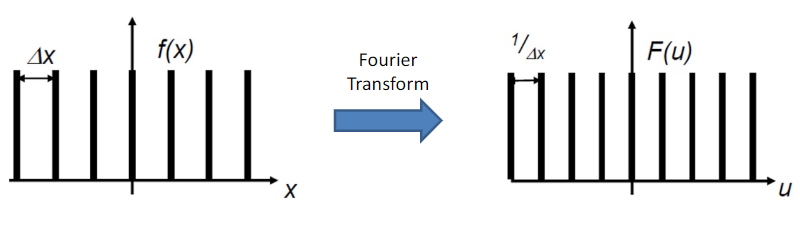
\includegraphics[width=0.38\textwidth]{Lec3/脉冲}
        \caption{a Dirac comb function}
    \end{figure}

    Sampling = Repeating Frequency Contents.
    \begin{figure}[H]
        \centering
        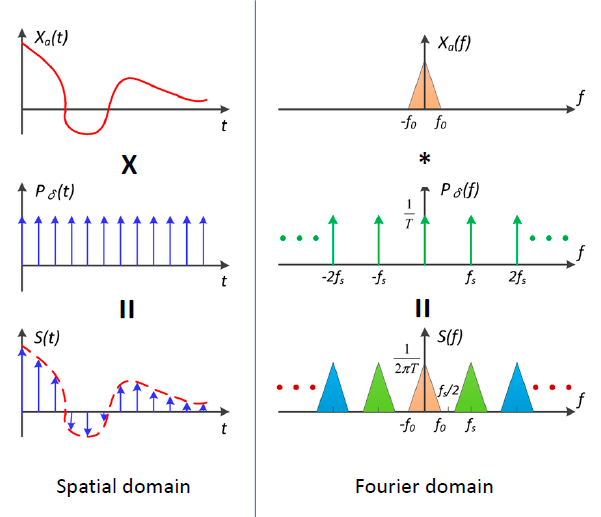
\includegraphics[width=0.38\textwidth]{Lec3/采样}
        \caption{Sampling}
    \end{figure}

    Aliasing = Mixed Frequency Contents(频谱混叠)
    \begin{figure}[H]
        \centering
        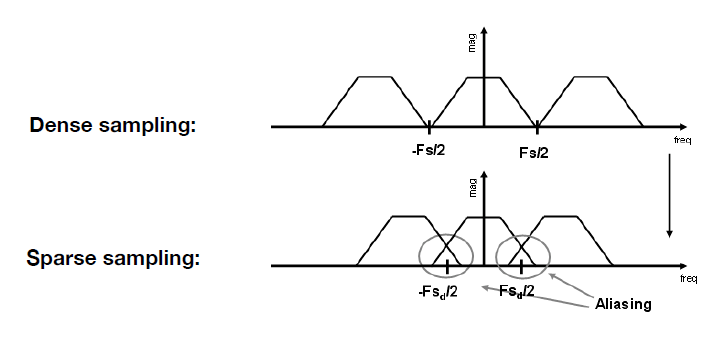
\includegraphics[width=0.38\textwidth]{Lec3/走样}
        \caption{Aliasing}
    \end{figure}
    可将高频信号过滤后采样

    
    \subsection{Nyquist-Shannon theorem(奈奎斯特采样定理)}
    由此可计算采样最小的频率.

    Consider a band-limited signal: has no frequencies above $f_0$.

    The signal can be perfectly reconstructed if sampled with a frequency larger than $2f_0$.

    由此Anti-alisaing = Filtering, then Sampling.
    \begin{enumerate}
        \item Convolve the image with low-pass filters (e.g. Gaussian)
        \item Sample it with a Nyquist rate
    \end{enumerate}
    \begin{figure}[H]
        \centering
        \begin{subfigure}{0.36\textwidth}
            \centering
            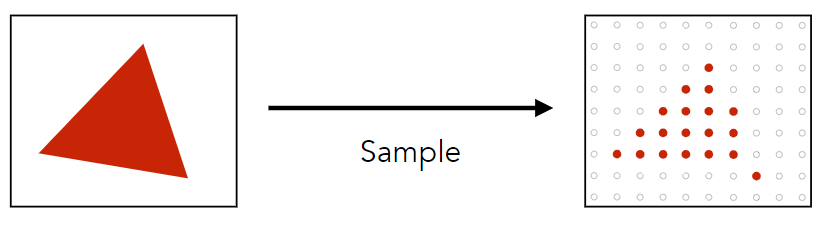
\includegraphics[width=\textwidth]{Lec3/regular sampling}
            \caption{Regular Sampling}
        \end{subfigure}
        \begin{subfigure}{0.36\textwidth}
            \centering
            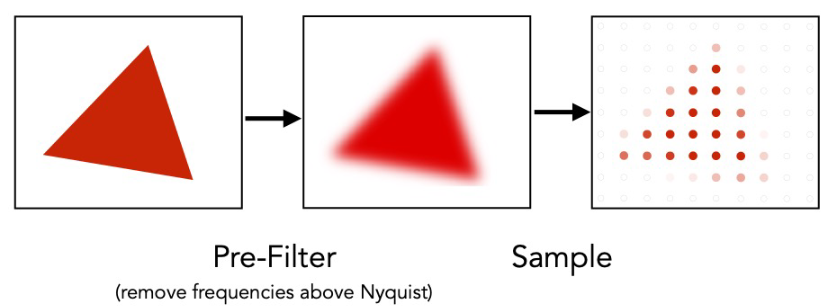
\includegraphics[width=\textwidth]{Lec3/antialiased sampling}
            \caption{Anti-aliased Sampling}
        \end{subfigure}
    \end{figure}

\section{Image magnification}

\subsection{Interpolation(插值)}
一维
\begin{enumerate}
    \item Nearest-neighbor interpolation(最近邻)
    
    Not continuous, not smooth
    \begin{figure}[H]
        \centering
        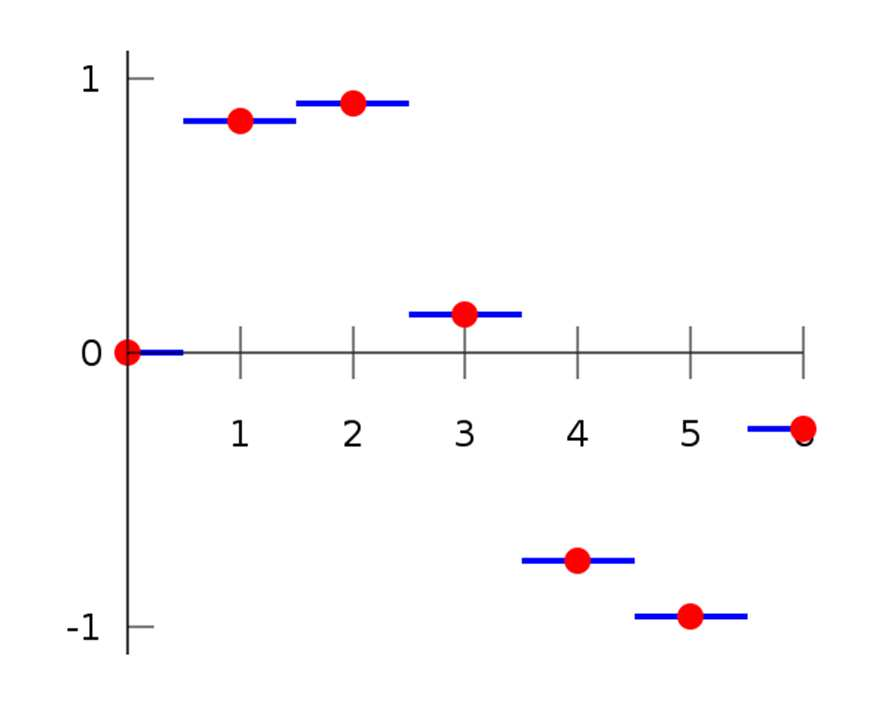
\includegraphics[width=0.22\textwidth]{Lec3/Nearest-neighbor}
        \caption{Nearest-neighbor interpolation}
    \end{figure}
    \item Linear interpolation(线性)
    
    Continuous, not smooth
    \begin{figure}[H]
        \centering
        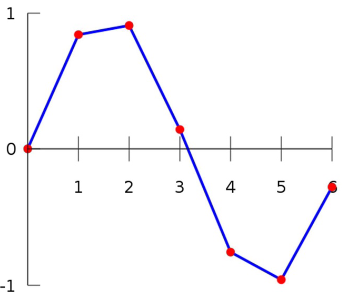
\includegraphics[width=0.22\textwidth]{Lec3/Linear}
        \caption{Linear interpolation}
    \end{figure}
    
    \item Cubic interpolation(三次多项式, 三次样条)
    
    Continuous, smooth
    \begin{figure}[H]
        \centering
        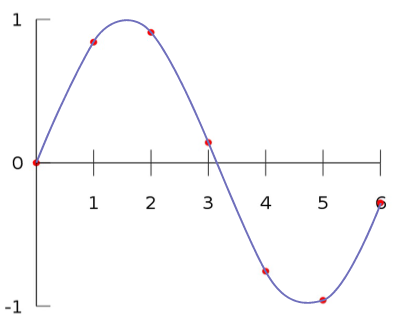
\includegraphics[width=0.22\textwidth]{Lec3/Cubic}
        \caption{Cubic interpolation}
    \end{figure}
    For each interval: $y=ax^3+bx^2+cx+d$(每一段一个多项式)
\end{enumerate}
二维
\begin{enumerate}
    \item Bilinear Interpolation
    
    将二维插值转换为几次一维的插值, 一般用这个, generally bilinear is good enough
    \begin{figure}[H]
        \centering
        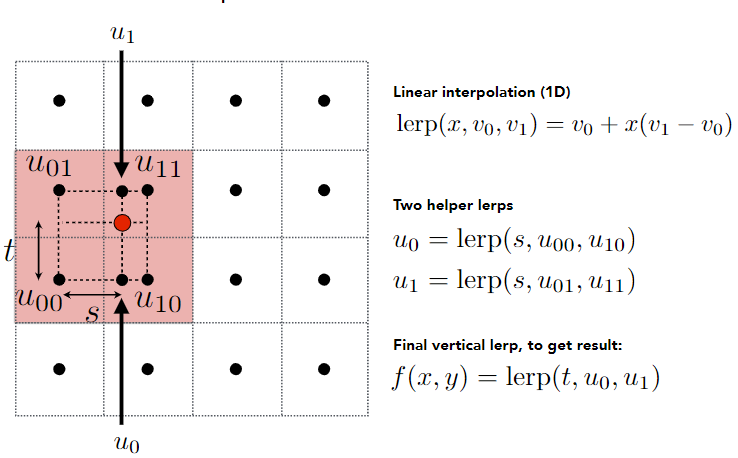
\includegraphics[width=0.38\textwidth]{Lec3/Bilinear}
        \caption{Bilinear interpolation}
    \end{figure}

    \item Bicubic Interpolation
    
    $p(x,y)=\sum_{i=0}^{3}\sum_{j=0}^{3}a_{ij}x^iy^j$

\end{enumerate}
Super-Resolution(超分辨率):神经网络

\subsection{Seam Carving for Content-Aware Image Resizing(有内容的裁剪)}
\begin{enumerate}
    \item Basic idea: (裁掉变化小的地方)remove unimportant pixels
    \item Important of pixel: edges are important. Egde energy $E(I)=\left|\frac{\partial I}{\partial x}\right|+\left|\frac{\partial I}{\partial y}\right|$
    
    方式: 用边缘检测滤波做卷积(相当于获得梯度)后相加, 即可得到Egde energy图像.

    eg:
    \begin{figure}[H]
        \centering
        \begin{subfigure}{0.38\textwidth}
            \centering
            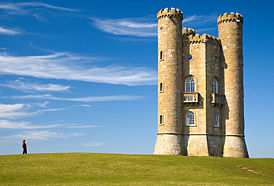
\includegraphics[width=\textwidth]{Lec3/Egde energy pre}
            \caption{Egde energy pre}
        \end{subfigure}
        \begin{subfigure}{0.38\textwidth}
            \centering
            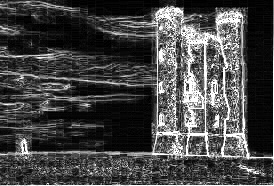
\includegraphics[width=\textwidth]{Lec3/Egde energy}
            \caption{Egde energy}
        \end{subfigure}
    \end{figure}
    \item Seam carving: Find connected path of pixels from top to bottom of which the edge energy is minima(除去的是连续的一条曲线, 且梯度最小)
    \begin{figure}[H]
        \centering
        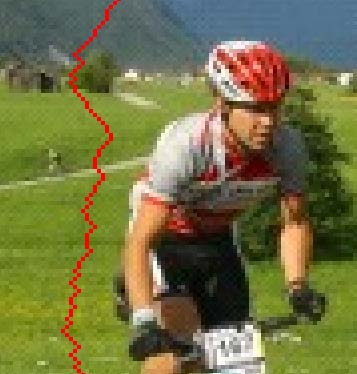
\includegraphics[width=0.22\textwidth]{Lec3/seam}
        \caption{seam}
    \end{figure}
    方式: DP $M(i,j)$代表从上到下经过这个点的最小梯度, 有$M(i,j)=E(i,j)+\min(M(i-1,j-1),M(i-1,j),M(i-1,j+1))$
\end{enumerate}

\subsection{Seam insertion(接缝插值)}
Find k seams to insert. Then interpolate pixels.

eg:
\begin{figure}[H]
    \centering
    \begin{subfigure}{0.38\textwidth}
        \centering
        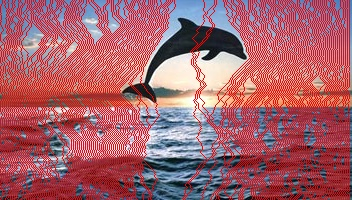
\includegraphics[width=\textwidth]{Lec3/Seam insertion pre}
        \caption{Seam insertion pre}
    \end{subfigure}
    \begin{subfigure}{0.38\textwidth}
        \centering
        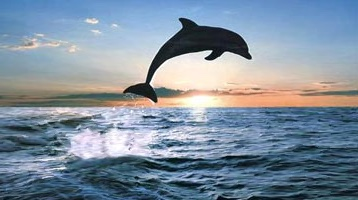
\includegraphics[width=\textwidth]{Lec3/Seam insertion}
        \caption{Seam insertion}
    \end{subfigure}
\end{figure}